
%!TEX ROOT=../_main.tex

\chapter{Tvarova optimalizace kompresorove mrize}

Optimalizace kompresorové mříže je fajn

Obecny popis pripadu a OP
2D

\section{Obecný popis problému}

Simulace prováděné v rámci této práce zjednodušeně reprezentují měřící soustavu tzv. lopatkových mříží. Pro lopatkové mříže jsou určující zejména geometrie samotné lopatky, rozteč $ t $ jednotlivých lopatek a stav proudu před a za mříží.

V rámci numerické simulace je topologie výpočetní oblasti naznačena na obrázku \ref{fig:vypocetni_oblast}. Vstupní a výstupní hranice jsou rovnoběžné s osou y a jejich výška je právě zmiňovaný parametr rozteče $ t $. Uprostřed oblasti se nachází uzavřená hranice reprezentující geometrii lopatky. Vrchní a spodní hranice jsou brány jako periodické, tedy to co vyteče spodem, vteče vrchem a naopak. Prostorová diskretizace (síť) je v této práci vždy dělána tak, aby si stěny buněk na obou stranách periodické hranice odpovídali $ 1:1 $, pouze s posunutím $ t $.

\begin{figure}
	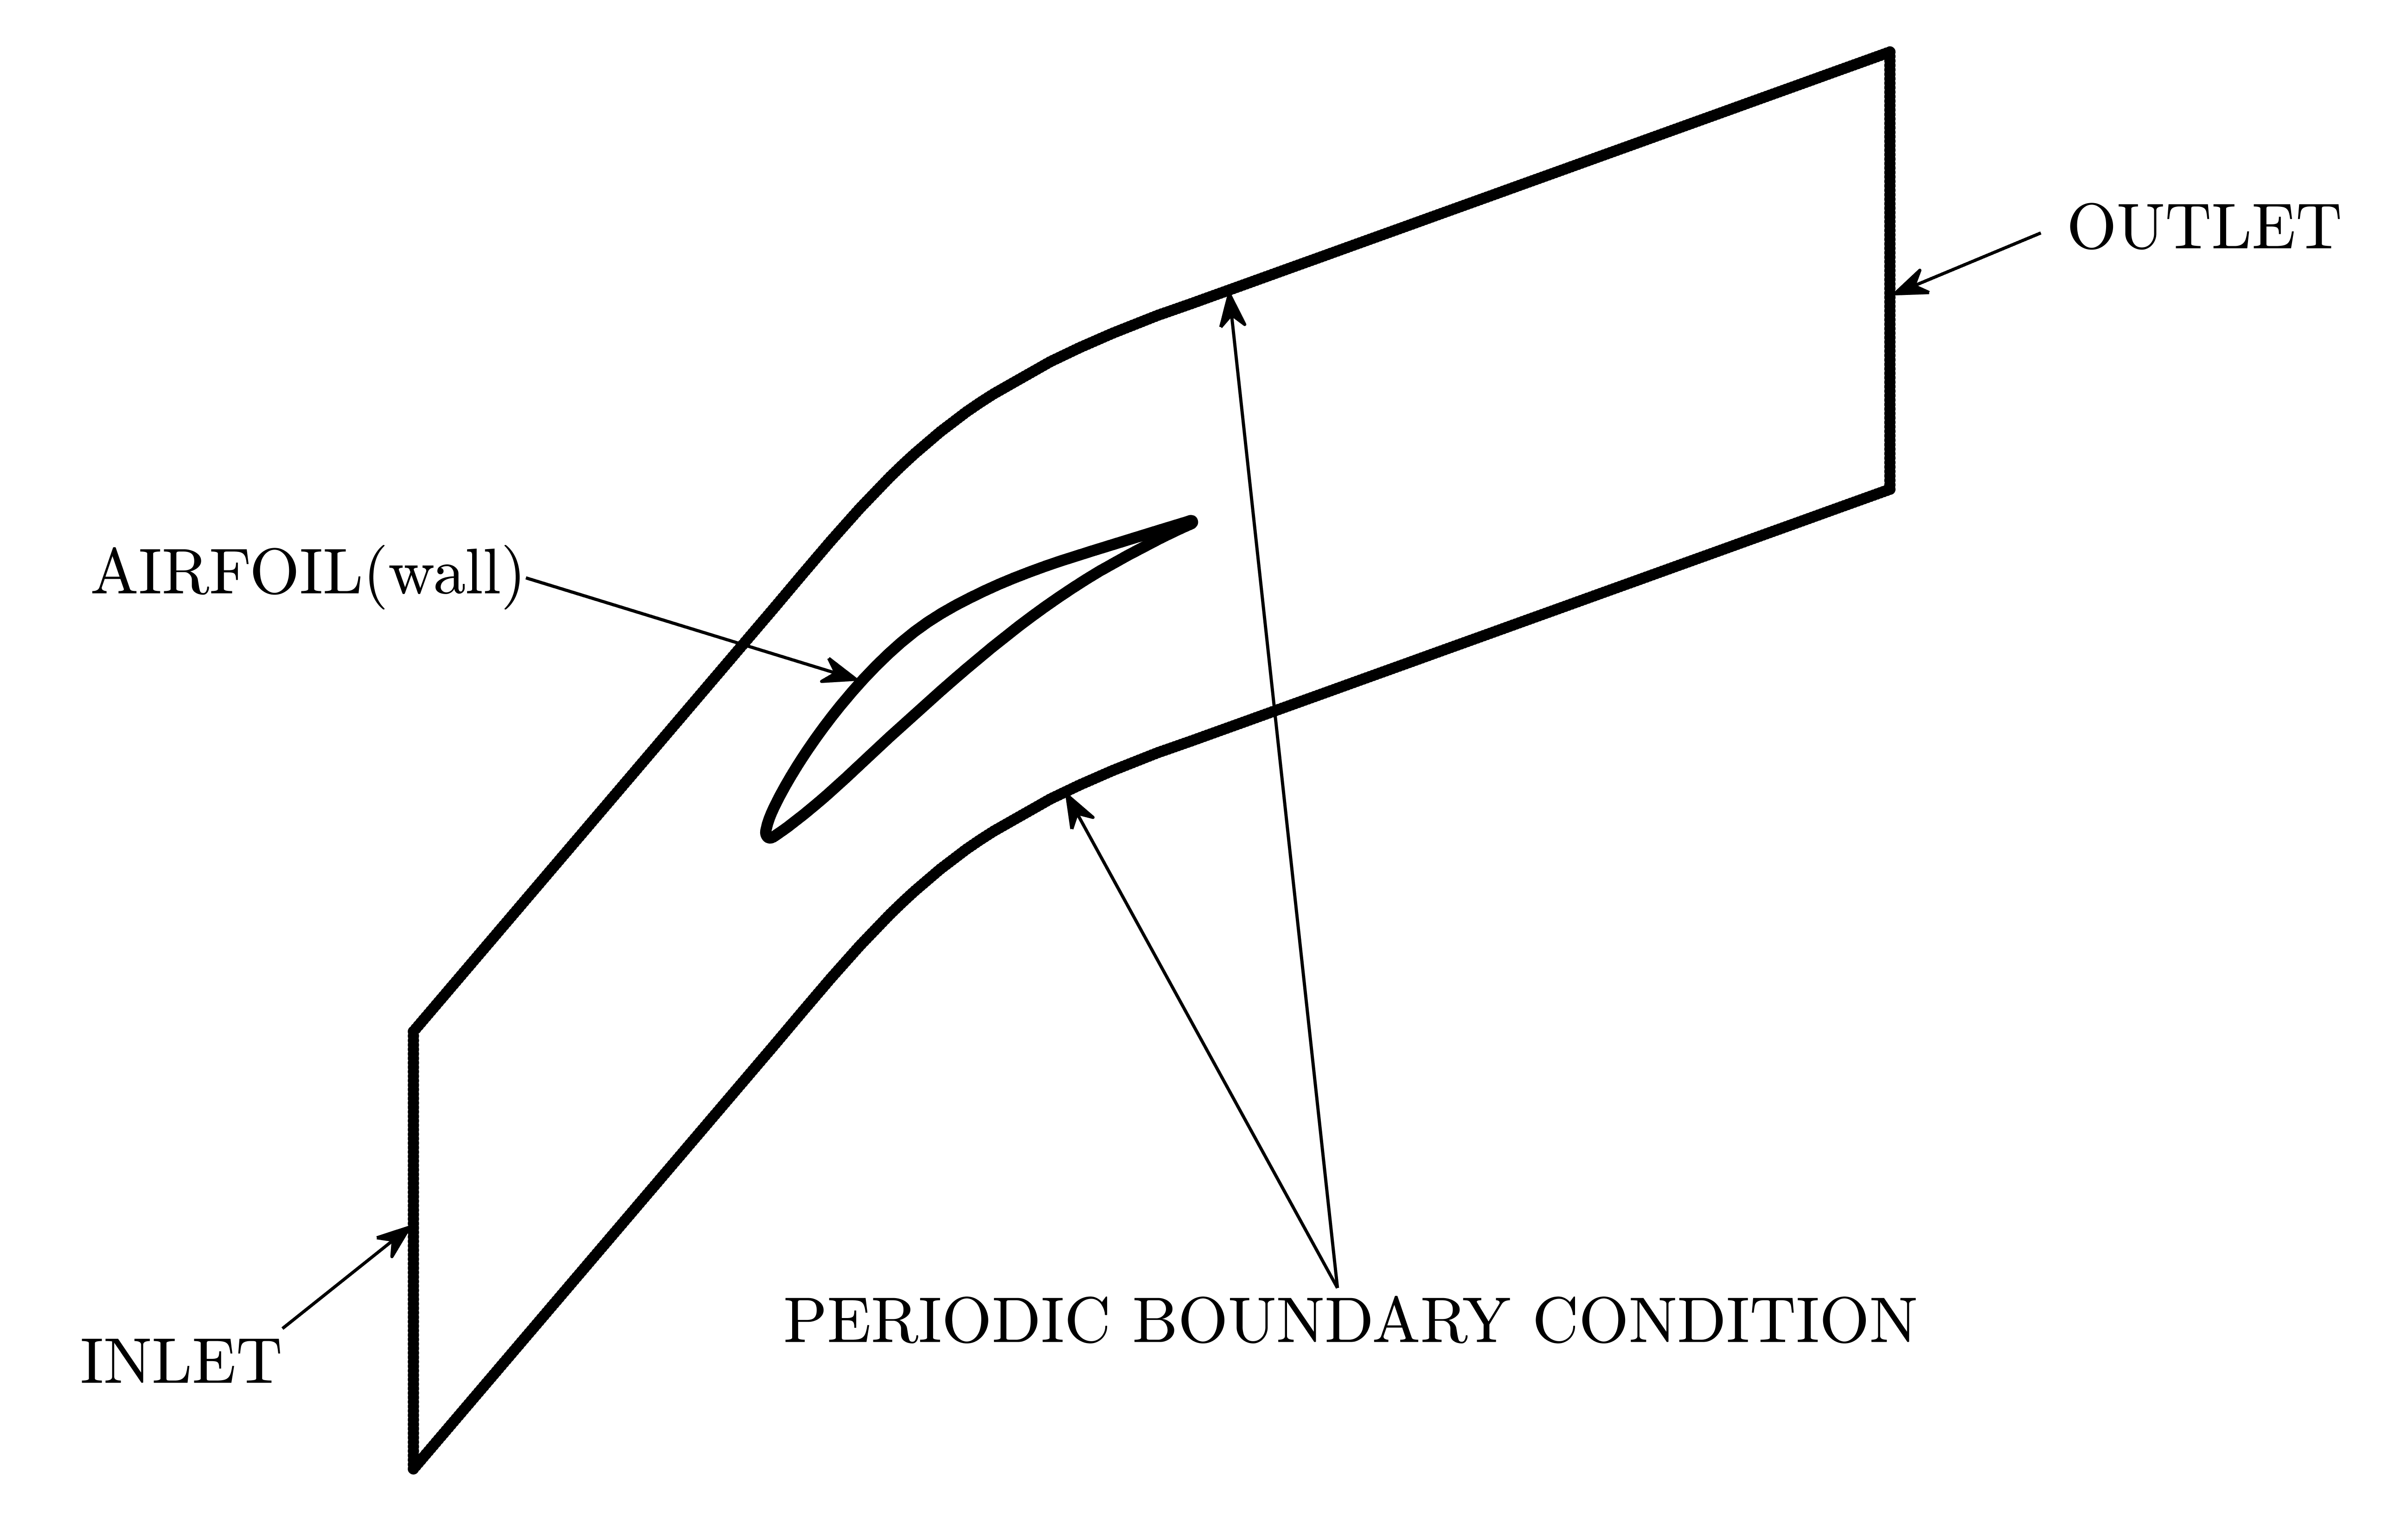
\includegraphics[width=0.7\textwidth]{img/ComputationalDomain.png}
	\caption{Náčrt topologie výpočetní oblasti pro standardní axiální kompresorovou mříž.}
	\label{fig:vypocetni_oblast}
\end{figure}

Krom periodicity jsou další okrajové podmínky následující. Na vstupu je předepsána Dirichletova okrajová podmínka pro vektor rychlosti a turbulentní proměnné. Tlak zde má nulovou Neumanovu podmínku. Na výstupu je naopak statický tlak fixován na nulu a rychlost je zde předepsána pomocí nulového gradientu.

\section{Cílové funkce}

V rámci aplikace sdružené optimalizace na tvar lopatky kompresorové mříže lze vymyslet hned několik cílů. V jednom stupni axiálního kompresoru se běžně sledují veličiny stlačení, účinnost (respektive ztráty) a výstupní úhel proudu. Pro tuto práci se jako sledovaná a optimalizovaná veličina bere ta poslední, tedy výstupní úhel proudu $ \alpha_2 $. 

K dosažení cílového úhlu na výstupu z lopatkové mříže $ \alpha_{2tar} $ jsou použity dva postupy. Oba vycházejí z definice úhlu výstupního proudu
\begin{equation}
\alpha_2 = \arctan\left(\dfrac{u_{y2}}{u_{x2}}\right).
\end{equation}
Ze zákona zachování hmotnosti pro proudění nestlačitelné tekutiny vyplývá, že to co do kontrolní oblasti vteče, musí i vytéct. Jinými slovy toky vstupní a výstupní hranicí se musejí rovnat
\begin{equation}
\dot{m_1}=\dot{m_2},
\end{equation}
což pro proudění nestlačitelné tekutiny kontrolní oblastí s vstupní a výstupní hranicí rovnoběžnou s osou y znamená, že 
\begin{equation}
u_{x1}=u_{x2}.
\end{equation}
Okrajové podmínky definují na vstupu konstantní uniformní vektor rychlosti $ \mathbf{u_1} $ a přeneseně tedy i x-ovou složku rychlosti na výstupu. Z toho vyplývá, že pro zadané $ \alpha_{2tar} $ můžeme apriori spočítat
\begin{equation}
u_{y2tar} = \tan(\alpha_{2tar}) \cdot u_{x2},
\end{equation}
tedy jistou cílovou rychlost na výstupu a cílovou funkci formulovat pomocí ní.

Dále jsou srovnány dvě formulace cílové funkce. První formulace optimalizuje přímo výstupní složku rychlosti, kdežto druhá optimalizuje nepřímo přes sílu na lopatku.

\subsection{Přímá formulace}

V přímé formulaci se snažíme aby
\begin{equation}
	u_{y2tar}=\dfrac{1}{\phi_2}\sum_{f\in\Gamma_2}\phi_f u_{yf},
\end{equation}
tedy aby průměr $ u_y $ na výstupu vážený přes hmotnostní tok byl roven zadané cílové rychlosti.
Minimalizovanou cílovou funkci formulujeme jako
\begin{equation}
	J = \int_{\Gamma_2}\left( u_y(y)-u_{y2tar} \right)^2\mathrm{d}S = \int_{\Gamma_2} J_\Gamma\, \mathrm{d}S.
\end{equation}
Ve smyslu vztahu \ref{eq:cenova_fce} má takto definovaná cílová funkce pouze hraniční složku $ J_\Gamma $ a pro sdružené rovnice tak bude ;ovat pouze v hraničních členech, tedy v rovnicích \ref{eq:sdruzenaOP1} a \ref{eq:sdruzenaOP2}. Potřebujeme tedy vydefinovat parciální derivace podle primárních proměnných $ \mathbf{u} $ a $ p $. Pro implementaci v rámci knihovny OpenFOAM je pak navíc potřeba vydefinovat ještě derivace podle $ u_n $ a $ u_t $, což pro dříve definovanou úlohu znamená podle složek $ u_x $ a $ u_y $.

Parciální derivace podle primárního tlaku $ \dfrac{\partial}{\partial p} $ je nulová, neboť tlak v cílové funkci nefiguruje.

Pro parciální derivaci podle primární rychlosti $ \mathbf{u} $ je lepší se dívat na složku $ u_y $ jako na skalární součin $ \mathbf{u}\cdot \mathbf{j}=\mathbf{u}\cdot (0,1,0) = u_y$ a derivaci tedy provést jako
\begin{equation}\label{key}
\dfrac{\partial J_\Gamma}{\partial \mathbf{u}}
=
\dfrac{\partial \left( \mathbf{u}\cdot \mathbf{j}-u_{y2tar} \right)^2}{\partial \mathbf{u}}
=
2( \mathbf{u}\cdot \mathbf{j}-u_{y2tar} )\,\mathbf{j}
=
2( u_y-u_{y2tar} )\,\mathbf{j}.
\end{equation}
U dodatečných derivací pro OpenFOAM vychází $ \dfrac{\partial}{\partial u_n}=0 $ a $ \dfrac{\partial }{\partial u_t} $ je stejná jako derivace podle $ \mathbf{u} $.

implementace v OF do apendixu?

\subsection{Nepřímá formulace přes sílu}

Druhou možností jak dosáhnout zadaného úhlu výstupního proudu je použít optimalizaci přes cílovou sílu. 
Optimalizace síly na stěnu ve smyslu její minimalizace v předepsaném směru je v balíku OpenFOAM formulována jako
\begin{equation}\label{key}
J=\dfrac{\int_\Gamma \rho (-\tau_{ij}n_j+pn_i)r_i\,\mathrm{d}S}{\frac{1}{2}\rho A U_{\infty}^2},
\end{equation}
kde $ \tau_{ij} $ jsou složky tenzoru napětí, $ p $ tlak dělený konstantní hustotou $ \rho $ a $ \mathbf{n} $ jednotkový normálový vektor. Vektor $ \mathbf{r} $ pak definuje směr projekce vektoru síly (směr ve kterém se minimalizuje). $ A $ je referenční plocha a $ U_{\infty} $ je rychlost volného proudu. Takto definovaná cílová funkce tedy svou velikostí odpovídá koeficientu síly $ C_f $.¨

Zatímco přímá formulace ovlivňovala přes derivaci cílové funkce okrajovou podmínku sdružených pouze na výstupní hranici, cílová funkce přes sílu ovlivňuje okrajovou podmínku přímo na lopatce. Druhým rozdílem je pak, že v přímé formulaci se objevuje jediná primární proměnná, kdežto pro integraci síly na lopatce jsou potřeba všechny proměnné, včetně turbulentní proměnné $ \widetilde{\nu} $. Tyto rozdíly zavdávají dostatečný důvod pro porovnání těchto dvou formulací ve smyslu rychlosti konvergence či přesnosti.


\section{Optimalizace mrize GHH 1-S1}

popis geometrie, vypocetni oblasti, okrajove podminky, nastaveni optimalizacniho algoritmu

Pro aplikaci optimalizačního algoritmu s novou cenovou funkcí pro stlačení byla zvolena axiální kompresorová mříž MAN GHH 1-S1 publikovaná v \cite{steinert1990design}. Výpočetní oblast 

\subsection{vysledky}
klaibrace S-A modelu, prubeh cilove fce, overeni vysledku pomoci vhodnejsiho modelu turbulence
